\chapter{Исследовательский раздел}

%
\section{Апробация метода}

%%
\subsubsection{Подготовка данных}

Для исследования было принято решение использовать 3 блока данных:

\begin{itemize}
    \item 23 000 записей с сайта zona.media
    \item 1 000 000 записей с сайта ria.ru
    \item 24 000 случайно выбранных записей из 1 000 000 с сайта ria.ru
\end{itemize}

~\

Подготовка двух блоков данных по 23 и 24 тысячи записей происходила в один поток. Для обработки 1 миллиона записей была использована многопоточность. Записи были обработаны в 16 парааллельных потоков.

Так же были удалены слова, которые использовались меньше 10 раз и больше 2000 раз во всей коллекции, а так же слова, которые встречаются только в 0.01\% документов.

%%
\subsubsection{Подбор базовых значений коэффициентов регуляризации}

Что бы получить первые результаты исследования необходимо определить хотя бы примерно центры диапазонов коэффициентов при регуляризаторах для последующего их уточнения. После каждой попытки анализируется результат. Проверяется достиг ли исследователь своей цели по соответствующему параметру и не выродилась ли при этом модель.

Так как регуляризаторы добавляются последовательно, поиск базовых значений так же реализован последовательно. Сначала на коллекции обучается модель PLSA до тех пор, пока модель не сойдется. После этого добавляется первый регуляризатор, разреживающий матрицу слова-темы $\Phi$.

После обучения нескольких десятков первых моделей на 23 тысячах записей с zona.media были определены базовые значения коэффициентов регуляризации:

\begin{itemize}
    \item регуляризатор, разреживающий матрицу слова-темы $\Phi$: -3;
    \item регуляризатор, разреживающий матрицу темы-документы $\Theta$: -5;
    \item регуляризатор, увеличивающий разницу между ядрами тем: 25 000 000.
\end{itemize}

\begin{figure}[h]
    \center{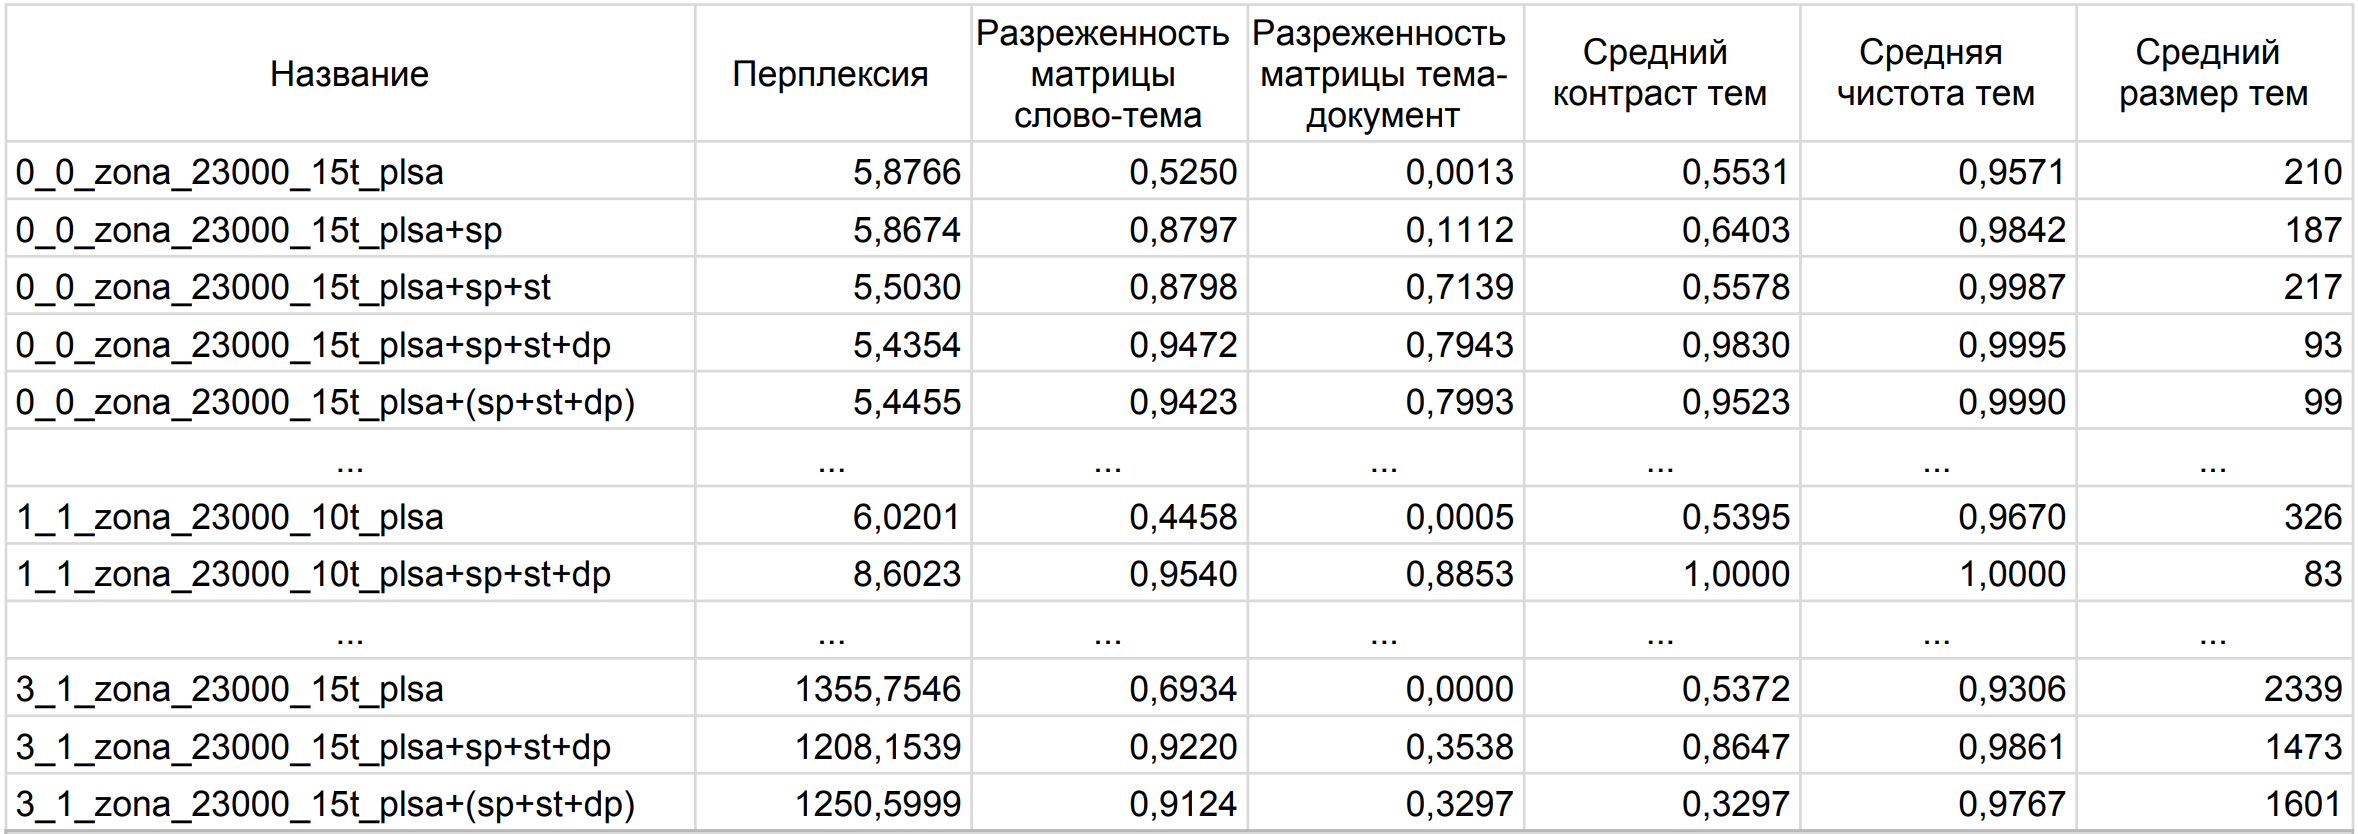
\includegraphics[scale=0.3]{res_table_1.png}}
    \caption{Стадия исследования коэффициентов регуляризации.}
    \label{fig:res_table_1}
\end{figure}

Из \todo{}рисунка \ref{fig:res_table_1} видно, что одновременное включение всех регуляризаторов приводит к худшим результатам, чем стратегия с подключением регуляризаторов по одному, и обучения последовательно до сходимости.
%%
\subsubsection{Определение оптимального количества тем}

После того, как были найдены приблизительные значения коэффициентов регуляризации было принято решение сменить коллекцию новостей на 24 тысячи случайно отобранных документов из 1 миллиона с сайта ria.ru, что бы темы стали еще более различны.

Было проведено исследование и построены следующие модели (рисунок \ref{fig:res_table_2}):

\noindent15 тем:
\todo[inline]{Вставить картинку}

\noindent50 тем:
\todo[inline]{Вставить картинку}

\noindent100 тем:
\todo[inline]{Вставить картинку}

\noindent150 тем:
\todo[inline]{Вставить картинку}

\begin{figure}[h]
    \center{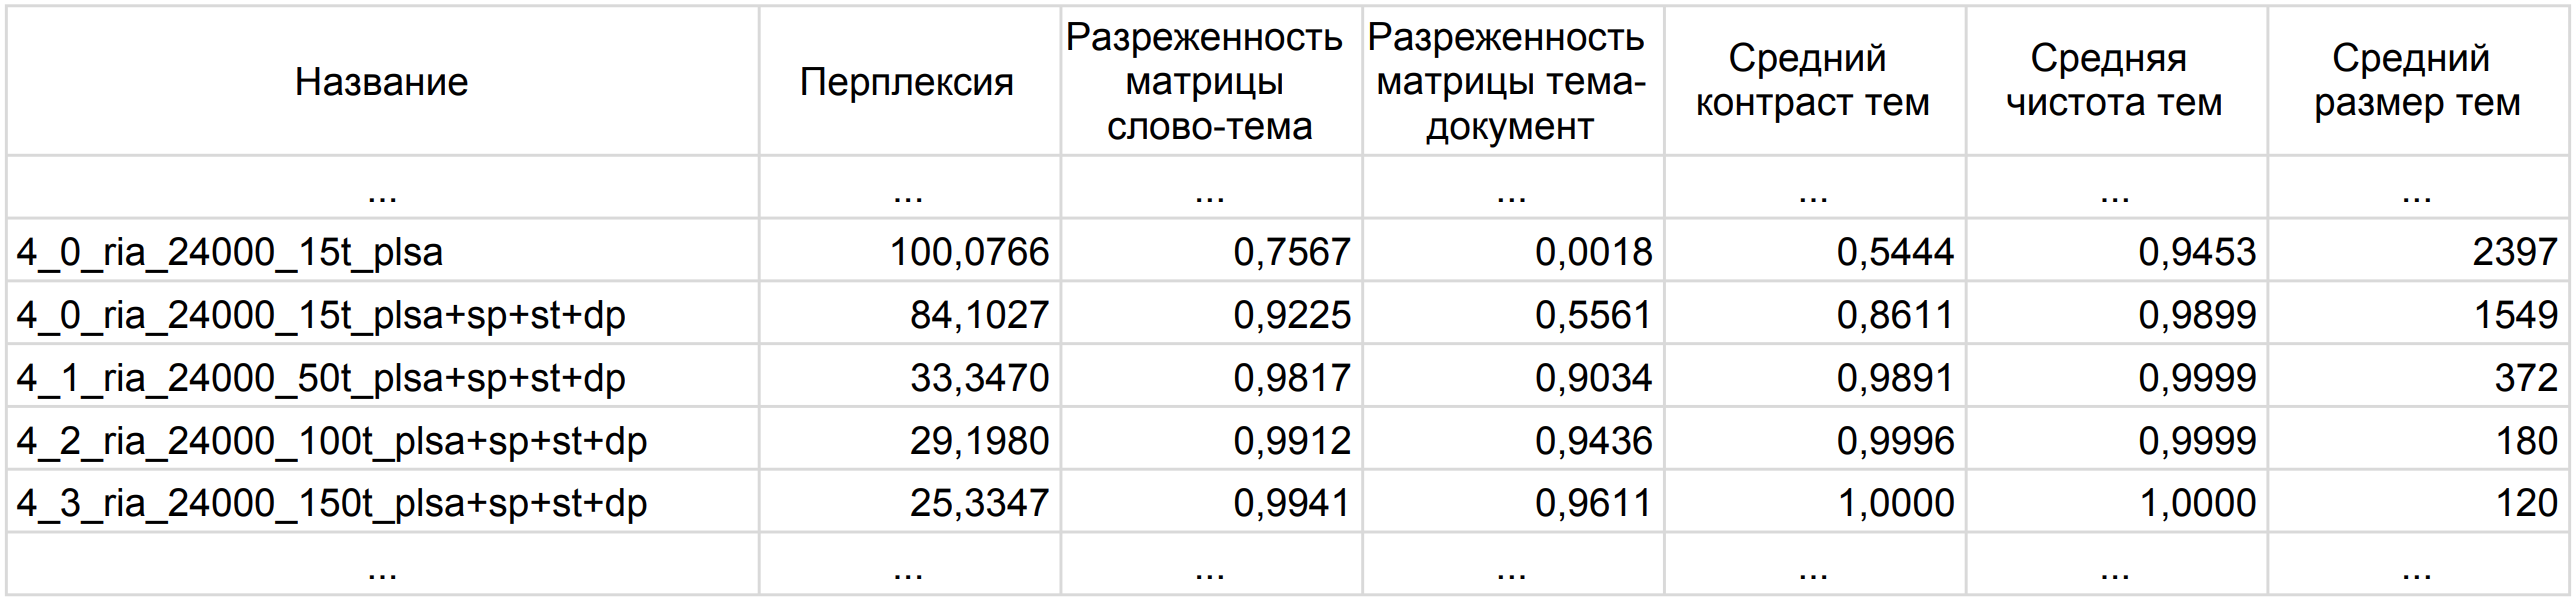
\includegraphics[scale=0.3]{res_table_2.png}}
    \caption{Стадия исследования коэффициентов регуляризации.}
    \label{fig:res_table_2}
\end{figure}

По каждой из модели были проанализированы топ 10 слов каждой из тем и проведена оценка. Каждая тема было отнесена к одной из двух категорий: тема состоит из характерных слов, понятно о чем она и для нее можно придумать название и тема состоит из несвязанных между собой слов, название придумать сложно.

Пример хороших тем:
\todo[inline]{Вставить список}

Пример плохих тем:
\todo[inline]{Вставить список}

Сравнительная таблица по 4 моделям:
\todo[inline]{Вставить сравнительную таблицу}

%
\section{Рекомендации}

\todo[inline]{}